\section{Affine algebraische Gruppen}
\label{sec:para1}
\subsection{Affine algebraische Varietät}
\label{sub:abschnitt_1.1}

\begin{defn}[Affine algebraische Menge]
	Sei $k = \overline{k}$ ein algebraisch abgeschlossener Körper,\marginnote{27.10.} $\aff_k^n := \{ (x_1,\dots,x_n) : x_i \in k\}$ sowie $I = (f_1,\dots,f_r) \subseteq k[x_1,\dots,x_n]$ ein Ideal. Wir bezeichnen
	\[ V(I) = \{x \in \aff_k^n : f(x) = 0 \text{ für } f \in I\} \]
	als \Index{affine algebraische Menge}.
\end{defn}

\begin{bsp}
	\begin{enumerate}[a)]
		\item Sei $f = \sum_{i=1}^{n} a_ix_i + c$ eine allgemeine lineare Gleichung, o.E. $a_1 \neq 0$. Dann ist $V(f)$ eine Hyperebene isomorph zu $\aff_k^{n-1}$. \\
		Im Fall $f=0$ ist $V(0) = \aff^n$ und im Fall $f = c \neq 0$ ist $V(c) = \emptyset$.
		\item Wir betrachten Quadriken. Sei $f$ quadratisch von der Gestalt
		\[ f = \underbrace{\sum_{1\leq i \leq j \leq n} a_{ij} x_i x_j}_{=: q \neq 0} + \underbrace{\sum_{x=1}^{n} b_i x_i}_{=: l} + c \]
		Idee: $f$ auf einfachere Gestalt bringen, z.B. mit $q$ in Diagonalform:
		\[ f = \sum_{i=1}^{n} a_i x_i + \sum_{i=1}^{n} b_i x_i + c \]
		mit $a_i \in \{0,1\}$ nach Skalierung. Koordinaten vertauschen:
		\[ f = \sum_{i=1}^{m} x_i^2 + \sum_{i=1}^{n} b_i x_i + c, \quad 1 \leq m \leq n \]
		Quadratische Ergänzung:
		\[ f = \sum_{i=1}^{m} x_i^2 + \sum_{i=m+1}^{n} b_i x_i + c \]
		Nun Beispiel a) anwenden:
		\[ f = \sum_{i=1}^{n} x_i^2 + c, c \in \{0,1\} \qquad \qquad \qquad f = \sum_{i=1}^{m} x_i^2 + x_n, m < n \]
		
		$n=2$:\todo{Das Wort "Skizze" sollte etwas höher stehen.} \\
		\begin{tabular}{rccc}
			& $x^2 + y^2 = 0$ & $x^2+y^2 = 1$ & $x^2 = y$ \\ 
			andere Varianten: & $x^2-y^2 = 0$ & $x^2-y^2=1$ &  \\ 
			Skizze: & 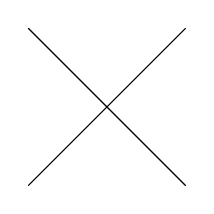
\begin{tikzpicture}
				\draw (-1,-1) -- (1,1);
				\draw (-1,1) -- (1,-1);
			\end{tikzpicture} & 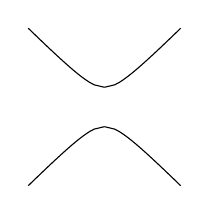
\begin{tikzpicture}[scale=0.5,rotate=90]
				\draw plot[domain=0.5:2] (\x,{(\x*\x-0.25)^(1/2)});
				\draw plot[domain=0.5:2] (\x,{-(\x*\x-0.25)^(1/2)});
				\draw plot[domain=-2:-0.5] (\x,{(\x*\x-0.25)^(1/2)});
				\draw plot[domain=-2:-0.5] (\x,{-(\x*\x-0.25)^(1/2)});
			\end{tikzpicture} & \begin{tikzpicture}[scale=0.5]
				\draw plot[domain=-2:2] (\x,{\x*\x});
			\end{tikzpicture} \\ 
			& zwei sich schneidende Geraden & Kreis (reell) bzw. Hyperbel (komplex) & Parabel
		\end{tabular} 
		
		$n = 3$: \todo{Hier fehlen drei Grafiken.}
		\[\begin{array}{ccc}
			x^2+y^2-z^2 = 0 & x^2+y^2-z^2=1 & x^2+y^2=z \\ 
			&  &   
		\end{array} \]
		Sei $f = x^2+y^2+z^2$ und $g = x^2+y^2+z$. \\
		\begin{equation}
		\begin{aligned}
			f(\vec{x_0} + t\vec{x}) &= (x_0 + tx)^2 + (y_0 + ty)^2 + (z_0 + tz)^2 \\
			&= 2t(x_0x+y_0y+z_0z) + x_0^2 + y_0^2 + z_0^2 + \text{ quad. Term} \\
			g(\vec{x_0}+t\vec{x}) &= 2t(x_0x+y_0y)+tz+x_0^2+y_0^2+ \text{ quad. Term}
		\end{aligned}
		\end{equation}
		\[ T_{(x_0,y_0,z_0)}Q = \{ (x,y,z) : \sprod{(x_0,y_0,z_0),(x,y,z)} = 0\} \qquad T_{(x_0,y_0,z_0)}Q = \{(x,y,z) : z = -2(x_0x + y_0y)\}\]
		\[ \dim T_{x_0}Q = \begin{cases}
			2 & (x_0,y_0,z_0) \neq 0 \\
			3 & (x_0,y_0,z_0) \neq 0
		\end{cases} \hspace{5cm}  \dim T_{x_0}Q = 2 \]
	\end{enumerate}
\end{bsp}
	
\subsection{Affine algebraische Varietät (ja, der Abschnitt hieß auch so!)}
\label{sub:abschnitt_1.2}
	$Z(I) := V(I)$		\marginnote{Bezeichnungen ändern sich aus irgendeinem nicht ersichtlichen Grund!} \\
	$a \subseteq S := k[x_1,\dots,x_n] \ni f_1, \dots, f_r, \quad I = (f_1,\dots, f_r)$ \\
	$T \subseteq S$ beliebige Teilmenge \\
	$Z(T) = \{p \in \aff^n : f(p) = 0 \text{ für alle } f \in T\}$ Nullstellenmenge
	
\begin{defn}
	Eine Teilmenge $Y \subseteq \aff^n$ heißt genau dann \bet{algebraisch}, falls $Y = Z(T)$ für eine Teilmenge $T \subseteq S$. \index{algebraische Teilmenge}
\end{defn}

\begin{satz}
	\begin{enumerate}[1)]
		\item $Z(T_1) \cup Z(T_2) = Z(T_1 \cdot T_2)$,
		\item $Z \enbrace*{\bigcup\limits_{i \in I} T_i} = \bigcap\limits_{i \in I} Z(T_i)$,
	\end{enumerate}
	d.h. die abgeschlossenen Teilmengen bilden eine Topologie.
\end{satz}

\begin{bsp}
	\begin{itemize}
		\item In $\aff^1$ sind die abgeschlossenen Teilmengen genau die endlichen Mengen und $\aff^1$.
		\item In $\aff^2$ sind die abgeschlossenen Teilmengen genau die endlichen Mengen, $\aff^2$ sowie endliche Vereinigungen $V(f_1) \cup \dots \cup V(f_r)$ (ohne Beweis)
		\item Die von den abgeschlossenen Mengen erzeugte Topologie ist nicht $T_2$: $p \in \aff^1$, $U \ni p$ offen, $Q \in \aff^1 \setminus U$, $V \supset Q$ offen $\Rightarrow U \cap V \neq \emptyset$.
	\end{itemize}
\end{bsp}
	
\begin{defn}[Irreduzibler topologischer Raum]
	Ein topologischer Raum $Y \neq \emptyset$ heißt \Index{irreduzibel}, falls gilt:
	\[Y = Y_1 \cup Y_2 \text{ mit } Y_1,Y_2 \text{ abgeschlossen} \quad \Rightarrow \quad Y_1 \subseteq Y_2 \text{ oder } Y_2 \subseteq Y_1 \]
\end{defn}

\begin{bsp}
	\begin{itemize}
		\item $\aff^1$ ist irreduzibel (später: $\aff^n$ ist irreduzibel)
		\item Folgende Quadriken sind irreduzibel: $f = X_1^2 + \dots + X_{n-1}^2 + X_n$ für $n \geq 1$, $f = X_1^2+ \dots + x_n^2 + 1$ für $n \geq 2$, $f = \sum_{i=1}^{n \geq 3} x_i^2$
		\item $V(x(x-1)) = \{ (0),(1) \}$ ist nicht irreduzibel.
		\item $x_1^2 + 1$, $x_1^2+x_2^2 = 0$ sind nicht irreduzibel
		\item $Y \subseteq X$ irreduzibel (mit induzierter Topologie) $\Rightarrow \overline{Y}$ irreduzibel.
	\end{itemize}
\end{bsp}

